% This is samplepaper.tex, a sample chapter demonstrating the
% LLNCS macro package for Springer Computer Science proceedings;
% Version 2.20 of 2017/10/04
%
\documentclass[runningheads]{llncs}
%
\usepackage{graphicx}
% Used for displaying a sample figure. If possible, figure files should
% be included in EPS format.
%
% If you use the hyperref package, please uncomment the following line
% to display URLs in blue roman font according to Springer's eBook style:
% \renewcommand\UrlFont{\color{blue}\rmfamily}

\begin{document}
%
\title{Simplex vs. Montecarlo, a brief comparision.\thanks{Supported by Universidad Tecnológica de Pereira.}}
%
%\titlerunning{Abbreviated paper title}
% If the paper title is too long for the running head, you can set
% an abbreviated paper title here
%
\author{Oscar Eduardo Bernal}
%
\authorrunning{O. Bernal}
% First names are abbreviated in the running head.
% If there are more than two authors, 'et al.' is used.
%
\institute{Universidad Tecnológia de Pereira, Colombia
\email{}}
%
\maketitle              % typeset the header of the contribution
%
\begin{abstract}
The Monte Carlo Method give us a process to solve big problems using randomness, by other side simplex is a method to solve linear optimization ploblems through an iterative process. Using HPC we can have an approach to parallel computing with a good amount of threads, but the Simplex method can't be easily parallelizable because in each iteration it depends of the previous state, while using Monte Carlo each step of the process is completely independient. Even so the question arises, is there really a difference between the Simplex method and the Monte Carlo method in a high-performance environment to solve linear optimization ploblems?

\keywords{HPC \and linear optimization \and Monte Carlo \and parallel computing \and Simplex}
\end{abstract}
%
%
%
\section{Introduction}
Es facil pensar en que un algoritmo puede ser mejor que otro, en especial cuando se trata de hacer tareas en paralelo, pero para poder lograr una comprension real de las implicaciones de una afirmación como esta se requiere, no solo un entendimiento de los algoritmos, si no tambien realizar un proceso de experimentacion, donde se pueda comprobar con datos reales la hipotesis planteada.

\subsection{Linear Optimization}
description of the broblems

\subsection{Simplex Method}
method description

\subsection{Monte Carlo Method}
whats up w tho method?

\subsection{Parallel computing}
whats up w tho method?

\subsection{Hipotesis}
Teniendo en cuenta la informacion sobre los dos metodos que se abordan en este documento se plantea la siguient hipotesis: 
Montecarlo es mejor que el metodo Simplex para solucionar problemas de Optimizacion Lineales con un gran numero de variables.

\section{Implementation}
Para poder poner a prueba esta hipotesis se desarrollaron 3 implementaciones, la primera y mas basica es una implementacion secuencial del metodo simplex, la segunda es una implementacion lineal del metodo montecarlo, y la ultima una version concurrente del metodo montecarlo.

\subsection{Sequential Simplex Method}
El metodo simplex parte de una matriz nx(m+n) donde n es el numero de variables del problema y m es el numero de restricciones, sobre esta matriz se empieza a iterar cambiando los valores de ciertas filas y columnas en cada iteracion, hasta que se encuentra la solucion.
Para evitar 

\subsection{Sequential Monte Carlo Method}
whats up w tho method?

\subsection{Parallel Monte Carlo Method}
whats up w tho method?

\section{Results}
put here something to say

\section{Conclusions}
put here something to say


%
%
%
%---------------- From here all are examlpe
%
%
%
\subsubsection{Sample Heading (Third Level)} Only two levels of
headings should be numbered. Lower level headings remain unnumbered;
they are formatted as run-in headings.

\paragraph{Sample Heading (Fourth Level)}
The contribution should contain no more than four levels of
headings. Table~\ref{tab1} gives a summary of all heading levels.

\begin{table}
\caption{Table captions should be placed above the
tables.}\label{tab1}
\begin{tabular}{|l|l|l|}
\hline
Heading level &  Example & Font size and style\\
\hline
Title (centered) &  {\Large\bfseries Lecture Notes} & 14 point, bold\\
1st-level heading &  {\large\bfseries 1 Introduction} & 12 point, bold\\
2nd-level heading & {\bfseries 2.1 Printing Area} & 10 point, bold\\
3rd-level heading & {\bfseries Run-in Heading in Bold.} Text follows & 10 point, bold\\
4th-level heading & {\itshape Lowest Level Heading.} Text follows & 10 point, italic\\
\hline
\end{tabular}
\end{table}


\noindent Displayed equations are centered and set on a separate
line.
\begin{equation}
x + y = z
\end{equation}
Please try to avoid rasterized images for line-art diagrams and
schemas. Whenever possible, use vector graphics instead (see
Fig.~\ref{fig1}).

\begin{figure}
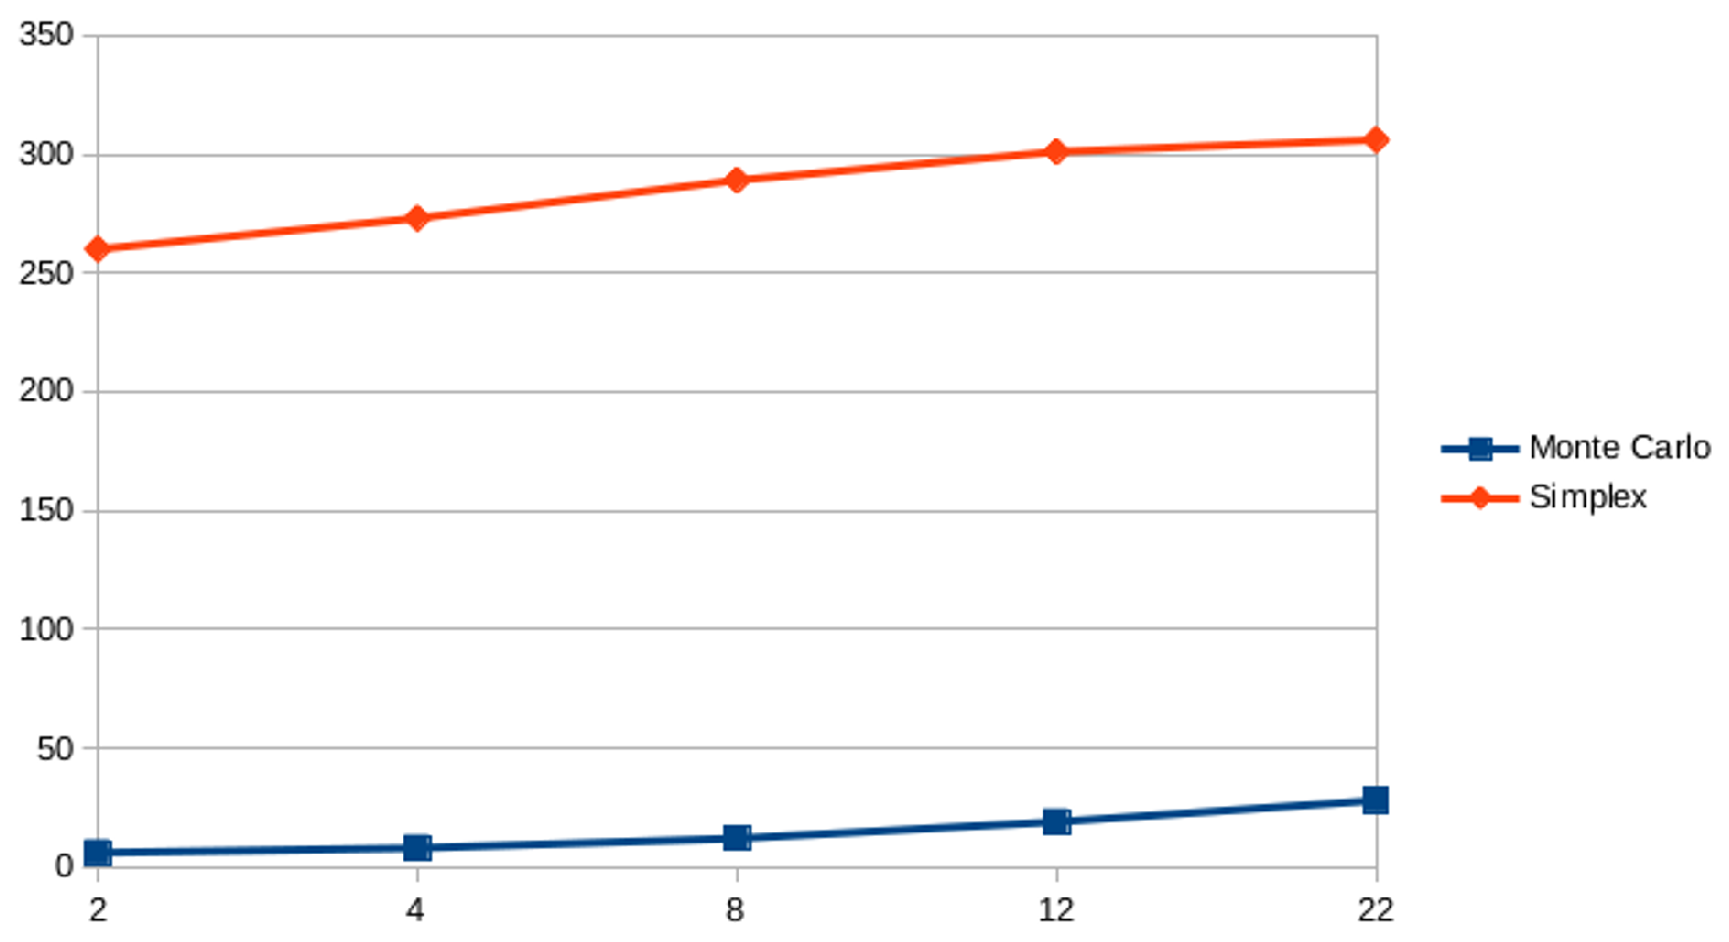
\includegraphics[width=\textwidth]{fig1.eps}
\caption{A figure caption is always placed below the illustration.
Please note that short captions are centered, while long ones are
justified by the macro package automatically.} \label{fig1}
\end{figure}

\begin{theorem}
This is a sample theorem. The run-in heading is set in bold, while
the following text appears in italics. Definitions, lemmas,
propositions, and corollaries are styled the same way.
\end{theorem}
%
% the environments 'definition', 'lemma', 'proposition', 'corollary',
% 'remark', and 'example' are defined in the LLNCS documentclass as well.
%
\begin{proof}
Proofs, examples, and remarks have the initial word in italics,
while the following text appears in normal font.
\end{proof}
For citations of references, we prefer the use of square brackets
and consecutive numbers. Citations using labels or the author/year
convention are also acceptable. The following bibliography provides
a sample reference list with entries for journal
articles~\cite{ref_article1}, an LNCS chapter~\cite{ref_lncs1}, a
book~\cite{ref_book1}, proceedings without editors~\cite{ref_proc1},
and a homepage~\cite{ref_url1}. Multiple citations are grouped
\cite{ref_article1,ref_lncs1,ref_book1},
\cite{ref_article1,ref_book1,ref_proc1,ref_url1}.
%
% ---- Bibliography ----
%
% BibTeX users should specify bibliography style 'splncs04'.
% References will then be sorted and formatted in the correct style.
%
% \bibliographystyle{splncs04}
% \bibliography{mybibliography}
%
\begin{thebibliography}{8}
\bibitem{ref_article1}
Author, F.: Article title. Journal \textbf{2}(5), 99--110 (2016)

\bibitem{ref_lncs1}
Author, F., Author, S.: Title of a proceedings paper. In: Editor,
F., Editor, S. (eds.) CONFERENCE 2016, LNCS, vol. 9999, pp. 1--13.
Springer, Heidelberg (2016). \doi{10.10007/1234567890}

\bibitem{ref_book1}
Author, F., Author, S., Author, T.: Book title. 2nd edn. Publisher,
Location (1999)

\bibitem{ref_proc1}
Author, A.-B.: Contribution title. In: 9th International Proceedings
on Proceedings, pp. 1--2. Publisher, Location (2010)

\bibitem{ref_url1}
LNCS Homepage, \url{http://www.springer.com/lncs}. Last accessed 4
Oct 2017
\end{thebibliography}
\end{document}
